%
% Hauptdatei
%


\documentclass[pdftex,a4paper,12pt,DIV15,BCOR20mm,parskip,numbers=noenddot]{scrbook}

	\usepackage{german, ngerman} %Deutsche Trennungen, Anf�hrungsstriche und mehr
	\usepackage[ngerman,german]{babel} % dt. Sprache laden (u.a. auch Ausgabe feststehender Begriffe in deutsch wie etwa Inhaltsverzeichnis statt table of contents)
	\usepackage[latin1]{inputenc} % Zeichenkodierung laden f�r Unix/Windows-Systeme
	\usepackage[babel,german=quotes]{csquotes} % Deutsche Eingabe von �,�,�,� erlauben	
	\usepackage[T1]{fontenc}
  \usepackage[pdftex]{color} 
  \usepackage{setspace} % Das Paket setspace erm�glicht ein einfaches Umstellen von normalem, anderthalbfachen oder doppeltem Zeilenabstand.
  \usepackage{graphics} %Zum Einbinden von Grafiken
  \usepackage[pdftex]{graphicx}  
	\usepackage[final]{listings}  % erm�glicht die Darstellung von (Programm-)Quellcode in der Arbeit
  \usepackage{ae,aecompl}  % ben�tigt zur PDF-Erzeugung, vgl http://dsanta.users.ch/resources/type1.html
  \usepackage[normalem]{ulem} % erm�glicht das Unterstreichen von Text
  \usepackage{amsfonts} % ok-zeichen usw
  \usepackage{scrpage2}
  \usepackage{bibgerm}
  \usepackage{array} % f�r tabellen
  
  \usepackage{times}
  \usepackage{algorithm}
  \usepackage{xspace}
  \usepackage{algpseudocode}
  \usepackage{amsmath}
  
  \usepackage{pgfplots}
  \usepackage{pgfplotstable}
  \pgfplotsset{width=14cm,compat=1.9}
  \usepackage{tikz}
  \usepackage{filecontents}
  
  \usepackage{amsthm}
  \theoremstyle{definition}
  \newtheorem{bsp}{Beispiel}
  
  \usepackage[section]{placeins}
  
  \usepackage{forest}
  \tikzset{el style/.style={midway, font=\scriptsize, inner sep=+1pt, auto=right}}
  \forestset{angled/.style={
  		content/.expanded={\noexpand\textless\forestov{content}\noexpand\textgreater}}}
  
  \newcommand{\Eop}[3][\!]{#2#1\to#1#3}
  \newcommand{\Assign}[2]{\mbox{$#1\leftarrow #2$}}
  \newcommand{\Size}[1]{|#1|}
  \newcommand{\Upto}[0]{\textbf{upto}\xspace}
  \newcommand{\Subchar}[2]{#1[#2]}
  \newcommand{\Substring}[3]{#1[#2\ldots#3]}
  \newcommand{\Rtab}[1][j_{0}]{R_{#1}}
  \newcommand{\EDcol}[1]{E_{\mathsf{col}}^{#1}}
  \newcommand{\Rcol}[1]{\Rtab^{#1}}
  \newcommand{\Deletion}[2][\!]{\Eop[#1]{#2}{\varepsilon}}
  \newcommand{\Insertion}[2][\!]{\Eop[#1]{\varepsilon}{#2}}
  \newcommand{\Replacement}[3][\!]{\Eop[#1]{#2}{#3}}
  \newcommand{\Substitution}[3][\!]{\Eop[#1]{#2}{#3}}
  \newcommand{\Crosspoints}[0]{C}
  \newcommand{\EvalCPname}[0]{\textit{evaluatecrosspoints}}
  \newcommand{\Rounddown}[1]{\left\lfloor#1\right\rfloor}
  \newcommand{\Roundup}[1]{\left\lceil#1\right\rceil}
  \newcommand{\Evalallcolsname}[0]{\mathit{evaluateallcolumns}}
  \newcommand{\Evalallcols}[3]{\Evalallcolsname(E,R,#1,#2,#3)}
  \newcommand{\EvalCP}[4]{\EvalCPname(\Crosspoints,#1,#2,#3,#4)}

	% Beliebige Farben definieren (bei Bedarf auskommentieren und selbst benennen und festlegen)
%	\definecolor{hellblau}{RGB}{238,242,247}
	
	\usepackage{colortbl} % f�r farbige Tabellen
	\usepackage{longtable} % f�r mehrseitige Tabellen
%	\usepackage{booktabs} % f�r tabellen: baut \midrule, \toprule und \bottomrule ein
%	\setlength{\tabcolsep}{30pt} % in Tabellen: Padding des Spalten nach links und rechts
	\renewcommand{\arraystretch}{1.25} % in Tabellen: Padding des Textes nach oben und unten in Prozent

	% Benutzt man bestimmte Spaltendefinitionen (hier: Spaltentyp p mit 25% Breite) �fter, kann man diese hier auslagern und unter einem bestimmten Buchstaben (hier: A) speichern
%	\newcolumntype{A}{p{0.25\textwidth}} 

	\usepackage{nomencl} % Package f�r ein Abk�rzungsverzeichnis
	\renewcommand{\nomname}{Abk�rzungsverzeichnis} % Deutsche �berschrift
	\setlength{\nomlabelwidth}{.20\hsize} % Breite eines Eintrags
	\renewcommand{\nomlabel}[1]{#1 \dotfill} % Auff�llen mit Punkten
	\setlength{\nomitemsep}{-2\parsep} % Zeilenabstand verkleinern
	\makenomenclature  % Datenbank des Abk�rzungsverzeichnisses beim Kompilieren des Textes erzeugen

	% fuer Literaturverweise
	\usepackage[numbers,square]{natbib}
	\bibpunct{[}{]}{;}{a}{}{;} % Natbib konfigurieren, so da� im text [M�ller 2006] erscheint und keine runden Klammern o.�.
	\renewcommand{\cite}{\citep} % \cite zu \citep umwandeln, so dass im Text \cite{Mueller.2006} f�r Referenzen verwendet werden kann.
%	\usepackage{url} % damit im LitVZ auch so etwas wie 'M�ller 2006: Vortrag zum Thema XY (Powerpoint-Pr�sentation)' steht; (Dateiendungen werden also textuell repr�sentiert)

	%% Verhindert, dass im Literaturverzeichnis nach der Nennung von [Mueller 2006] die Seite umgebrochen wird und die Autoren + Buchtitel etc. auf der n�chsten Seite landen
	%% Es wurde daher \noparagraphbreak in der natdin.bst bei der Ausgabe der Elemente erg�nzt
	%% siehe http://groups.google.de/group/de.comp.text.tex/browse_thread/thread/9ca4c681e2063fbd/f7eb3eec044b058e
	\makeatletter
	\def\noparagraphbreak{\interlinepenalty10000
	  \@itempenalty-\@highpenalty}
	\makeatother 


	% Fu�noten werden im gesamten Dokument fortlaufend hochgez�hlt und nicht nur kapitelweise, vgl. http://www.golatex.de/nummerierung-der-fussnoten-durchgehend-im-gesamten-dokument-t2042.html
	\usepackage{chngcntr}
	\counterwithout{footnote}{chapter}

	\setlength{\emergencystretch}{1em} % F�r den Fall, dass Zeilen im 1. Anlauf nicht richtig umgebrochen werden k�nnen, einen 'Notfallraum' einrichten (vgl. http://www.golatex.de/overfull-boxes-in-latex-t1979.html) 

	% Definitionen werden mit Hilfe von 'dfn' eingeleitet und k�nnen somit zentral formatiert werden.
	\newtheorem{dfn}{Definition}
	
	% entnommen aus http://www.siart.de/typografie/latextipps.xhtml#floats
	\renewcommand{\floatpagefraction}{0.8} % gibt den Bruchteil einer Seite, die f�r Gleitobjekte benutzt wird, an, der erreicht werden muss, bevor eine neue Seite angefangen wird. (Standard: 0.5; d.h. wenn ein Bild 51% der Seite einnimmt, wird extra f�r dieses Bild eine ganze Seite reserviert --> unsch�n)
	\renewcommand{\topfraction}      {0.8}
	\renewcommand{\bottomfraction}   {0.5} % \topfraction / \bottomfraction, gibt den Bruchteil einer Seite an, bis zu dem Gleitobjekte oben bzw. unten angeordnet werden sollen.
	\renewcommand{\textfraction}     {0.15} % gibt den Bruchteil einer Seite an, der mit Text belegt werden k�nnen muss.
	\makeatletter
	  \setlength{\@fptop}{0pt} % Wenn ein Float-Objekt allein auf einer Seite steht, soll es am oberen Rand der Seite erscheinen und nicht vertikal zentriert
	\makeatother
	
	% schrift auf palatino umstellen
  \usepackage{palatino}
  \setkomafont{sectioning}{\normalcolor\bfseries}


	% PDF-Support einbinden und konfigurieren
  \usepackage[
  	pdfstartview={Fit},   
  	pdffitwindow=true,
  	colorlinks,
  	linkcolor=black,
  	anchorcolor=black,
  	citecolor=black,
  	urlcolor=black
  ]{hyperref}
  \hypersetup
  {
  	pdftitle     = {Diplomarbeit zum Thema XY},
  	pdfsubject   = {Universit�t Hamburg / Department Informatik / ITG / Diplomarbeit},
  	pdfauthor    = {Vorname Nachname},
  	pdfkeywords  = {Diplomarbeit, Universit�t Hamburg}, % Hier kann eine beliebige Liste von Schl�sselw�rtern eingegeben werden, die z.B. Windows zur Indexierung/Suche benutzt
  	plainpages   = false 
  }
 
   
  % Zeilenabstand
  \setstretch{1.24}   

	% Strafpunkte, die beim Seitenumbruch vergeben werden, falls die erste Zeile eines Absatzes allein auf der vorangehenden Seite verbleibt. vgl http://www.jr-x.de/publikationen/latex/tipps/zeilenumbruch.html
	\clubpenalty=150

	% Strafpunkte, die beim Seitenumbruch vergeben werden, falls die letzte Zeile gerade noch auf die n�chste Seite umgebrochen wird. vgl http://www.jr-x.de/publikationen/latex/tipps/zeilenumbruch.html
	\widowpenalty=150  

  % Pagestyle definieren (nach Martins Template)
	\defpagestyle{diplHeadings}
	{ % es folgt: Definition des Seitenkopfes: 
	  % obere Linie
		(0pt,0pt)
		% linke Seite
		{\upshape \rlap{\pagemark} \hfill \headmark \hfill} % auf einer linken Seite soll LINKS die Seitenzahl stehen und mittig die Headline (headmark)
		% rechte Seite
		{\upshape \hfill \headmark \hfill \llap{\pagemark}} % auf einer rechten Seite soll RECHTS die Seitenzahl stehen und mittig die Headline (headmark)
		% falls Layout "one page"
		{}
		% untere Line
		(\textwidth,1pt)
	}
	{ % es folgt: Definition des Seitenfu�es: Wir wollen lediglich eine schwarze, �ber die komplette Seite gehende Linie erzeugen
	  % obere Linie
		(\textwidth,1pt)
		% linke Seite
		{}
		% rechte Seite
		{}
		% falls Layout "one page"
		{}
		% untere Linie
		(0pt,0pt)
	}  
	% Pagestyle auch f�r Chapter-Anfang einrichten
	\renewcommand*{\chapterpagestyle}{diplHeadings}
	\renewcommand*{\chapterheadstartvskip}{\vspace*{-\topskip}}
	\automark[section]{chapter}


	% R�nder	
	\setlength{\textwidth}{15cm}        % Textbreite
	\setlength{\textheight}{24cm}       % Texth�he
	\setlength{\topmargin}{-12mm}       % oberer Rand
  
 
  % Listingsformatierung (Quelltexte)
  \definecolor{lightgrey}{rgb}{0.90,0.90,0.90}
  \lstloadlanguages{XML}
  \lstset{
    tabsize=2,
    escapeinside={(*@}{@*)},
    captionpos=t,
    framerule=0pt,
    backgroundcolor=\color{lightgrey},
    basicstyle=\small\ttfamily,
    keywordstyle=\small\bfseries,
    numbers=left,
    fontadjust
  }    
%
% EOF
%  % Einbinden der Konfigurationen

\begin{document}


%
% Titelseiten Datei
%

\begin{titlepage}

	% Fehler "destination with the same identifier" unterdr�cken...
  \setcounter{page}{-1}

	% Titelseite
	\begin{figure}[h]
		\begin{minipage}[b]{25mm}
			
\includegraphics[width=25mm,clip]{images/logo_uhh}
		\end{minipage}
		\begin{minipage}[b]{2mm}
			
\includegraphics[width=1mm,height=24mm]{images/greypixel}
		\end{minipage}
		\begin{minipage}[b]{12 cm}
			{\sffamily
				{\Large Universit�t Hamburg } \\
				Fakult�t f�r Mathematik,\\
				Informatik und Naturwissenschaften \\
				Department Informatik \\
			}
		\end{minipage}
	\end{figure}

	\vfill
	
	\begin{center}
		% Diplomarbeit 
		\noindent { \huge
			Bachelorarbeit \\
					}
		\vspace{14mm}
		% Titel
		\noindent \textbf{\Large
		  Speichereffiziente Methoden zur Repr�sentation \\
		  von paarweisen Sequenz-Alignments \\		  
		}
		\vspace{10mm}
		
		%\noindent {\large
		%(Option:) In Kooperation mit:
		
		%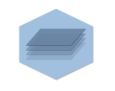
\includegraphics{images/logoitg.png}\\ %Firmenlogo
		%<Firma> \\
		%<Bereich / Abteilung>
		%}
	\end{center}
	
	\vfill
	
	\noindent \textbf{Thorben Wiese} \\
	\noindent \rule{\textwidth}{0.4mm} 
	\noindent{\textrm{3wiese@informatik.uni-hamburg.de}} \\
	\noindent{\textrm{Studiengang B.Sc. Informatik}} \\
	\noindent{\textrm{Matr.-Nr. 6537204}} \\
	\noindent{\textrm{Fachsemester 6}} \\
	\begin{tabbing}
	\hspace{20em} \=  \kill
	Erstgutachter Universit�t Hamburg: \> Prof. Dr. Stefan Kurtz \\
	Zweitgutachter Universit�t Hamburg: \> Dr. Giorgio Gonnella \\
		
	\hspace{20em} \=  \kill
	
	%(Option)Betreuer <Firma>: \> <Vorname> <Name> \\
			
	\end{tabbing}
	
	% R�ckseite der Titelseite mit Zitat
	\newpage 
	\thispagestyle{empty}
	\setcounter{page}{0}

	% wenn man Lust auf ein Zitat hat...
	% ... ansonsten auskommentieren
	~\\ \vfill \noindent 
%	A distributed system is one where the failure of some \\
%	computer I've never heard of can keep me from getting my work done. \\
%	\textit{-- Leslie Lamport}
\end{titlepage}

%
% EOF
%

% pagestyle umschalten
\pagestyle{diplHeadings}

\nomenclature{IT}{Informationstechnik}
\nomenclature{WWW}{World Wide Web} % Einbinden der zentralen Datei, die alle Abk�rzungen enth�lt
%
% Inhaltsverzeichnis
%

% --> Seitennummerierung r�misch
\pagenumbering{Roman}
\setcounter{page}{1}
\pdfbookmark[1]{Inhaltsverzeichnis}{toc}

\tableofcontents
%\cleardoublepage

%
% Abbildungs- und Tabellenverzeichnis
%
\listoffigures
\listoftables
%\cleardoublepage

%
% Abk�rzungsverzeichnis ausgeben
%
%\markboth{Abk�rzungsverzeichnis}{Abk�rzungsverzeichnis} % Kopfzeile anpassen, vgl. http://www.golatex.de/falsche-kopfzeile-im-abkuerzungsverzeichnis-t2074.html
%\printnomenclature % Abk�rzungsverzeichnis
%\cleardoublepage
%
% EOF
% % Inhalts-, Abbildungs-, Tabellenverzeichnis und Abk�rzungsverzeichnis laden (und ausgeben)

\pagenumbering{arabic}
\setcounter{page}{1}
\chapter{Einleitung}
%TODO ausf�hrlicher

Ein Sequenzalignment wird in der Bioinformatik dazu verwendet, zwei oder mehrere Sequenzen von zum Beispiel DNA-Str�ngen oder Proteinsequenzen miteinander zu vergleichen und die Verwandtschaft zu bestimmen. Ein Alignment ist das Ergebnis eines solchen Vergleichs. Bei einem globalen Alignment wird jeweils die gesamte Sequenz betrachtet, bei einem lokalen Alignment lediglich Teilabschnitte der beiden Sequenzen.
Um die verschiedenen Sequenzen vergleichen zu k�nnen, berechnet man einen Score oder die Kosten, um den Aufwand, den man betreiben muss, um die gegebenene Sequenz in die Zielsequenz umzuwandeln, beschreiben zu k�nnen. Hierbei wird jeweils das Optimum, also entweder der maximale Score oder die minimalen Kosten gesucht.
Die verschiedenen Schritte, um die Symbole der Strings zu ver�ndern, sind bei Gleichheit ein 'match', bei der Substitution ein 'mismatch', bei der L�schung eine 'deletion' und bei der Einf�gung eine 'insertion', welche je nach Verfahren unterschiedlich gewichtet werden k�nnen. Hierbei haben �hnliche Sequenzen einen hohen Score und geringe Kosten und unterschiedliche Sequenzen analog einen kleinen Score und hohe Kosten.

Ziel dieser Bachelorarbeit ist es, eine speichereffiziente Repr�sentation von paarweisen Sequenzalignments zu implementieren und die Funktionsweise, sowie Vergleiche zu anderen Verfahren zu diskutieren.

\section*{Die Edit-Operationen}

Die in diesem Kapitel eingef�hrten Begriffe werden in \cite[S. 5-7, 14-16]{gsa-skript} definiert.

Sei $\mathcal{A}$ eine endliche Menge von Buchstaben, die man Alphabet nennt. F�r DNA-Sequenzen verwendet man �blicherweise die Menge der Basen, also $\mathcal{A} = \{a, c, g, t\}$. $\mathcal{A}^i$ sei die Menge der Sequenzen der L�nge $i$ aus $\mathcal{A}$ und $\varepsilon$ sei die leere Sequenz. Formal ausgedr�ckt ist eine Edit-Operation ein Tupel 
\[(\alpha, \beta) \in (\mathcal{A}^1 \cup \{\varepsilon\}) \times (\mathcal{A}^1 \cup \{\varepsilon\}) \backslash \{(\varepsilon, \varepsilon)\},\]

Eine �quivalente Schreibweise von $(\alpha,\beta)$ ist $\alpha \rightarrow \beta$. Es gibt drei verschiedene Edit-Operationen
\begin{align*}
a \rightarrow \varepsilon &\indent \text{ ist eine Deletion f�r alle }a \in \mathcal{A}\\
\varepsilon \rightarrow b &\indent \text{ ist eine Insertion f�r alle }b \in \mathcal{A}\\
a \rightarrow b &\indent \text{ ist eine Substitution f�r alle }a,b \in \mathcal{A}
\end{align*}
Dabei ist zu beachten, dass $\varepsilon \rightarrow \varepsilon$ keine Edit-Operation darstellt.

Ein Alignment von zwei Sequenzen $u$ und $v$ l�sst sich nun als eine Sequenz $(\alpha_1 \rightarrow \beta_1, ... , \alpha_h \rightarrow \beta_h)$ von Edit-Operationen definieren, sodass $u = \alpha_1 ... \alpha_h$ und $v = \beta_1 ... \beta_h$ gilt.

\section*{Die Edit-Distanz}

Sei eine Kostenfunktion $\delta$ mit $\delta(a\rightarrow b)\geq 0$ f�r alle Substitutionen $a \rightarrow b$ und $\delta(\alpha \rightarrow \beta)>0$ f�r alle Einf�gungen und L�schungen $\alpha \rightarrow \beta$ gegeben. Die Kosten f�r ein Alignment $A = (\alpha_1 \rightarrow \beta_1, ... , \alpha_h \rightarrow \beta_h)$ ist die Summe der Kosten aller Edit-Operationen des Alignments.
\[\delta(A) = \sum_{i=1}^{h}\delta(\alpha_i \rightarrow \beta_i)\]
Ein Beispiel einer Kostenfunktion ist die Einheitskostenfunktion
\[
\delta(\alpha \rightarrow \beta) = 
\begin{cases} 
0 ,& \text{wenn } \alpha,\beta \in \mathcal{A} \text{ und } \alpha=\beta \\
1 , & \text{sonst.}
\end{cases}
\]
Die Edit-Distanz von zwei Sequenzen ist wie folgt definiert:
\[edist_\delta(u,v) = \min\{\delta(A) \mid A \text{ ist Alignment von }u \text{ und }v\}\]
Ein Alignment A ist optimal, wenn $\delta(A) = edist_\delta(u,v)$ gilt.\\[0,5cm]
Wenn $\delta$ die Einheitskostenfunktion ist, so ist $edist_\delta(u,v)$ die Levenshtein Distanz \cite[S. 19-21]{gsa-skript}.

Ein Alignment kann f�r eine Edit-Distanz $e$ mit der Einheitskostenfunktion in $O(e)$ Zeit berechnet werden \cite[S. 41-42]{gsa-skript}.

\chapter{Methoden}

\section{CIGAR-Strings}

Ein Dateiformat, welches zur Speicherung von Alignments verwendet wird, ist das SAM-Format oder die bin�r komprimierte Version BAM. Dieses codiert ein Alignment in einem sogenannten CIGAR-String der aus einzelnen Zeichen besteht, die jeweils eine Edit-Operation bezeichnen, also M f�r eine Substitution, I f�r eine Insertion und D f�r eine Deletion. Gleiche aufeinanderfolgende Operationen werden als Kombination von Quantit�t und Symbol geschrieben.

Sei $u =$ \texttt{actgaact}, $v =$ \texttt{actagaat} und das Alignment $A = (a\rightarrow a, c\rightarrow c, t\rightarrow t, ...)$ gegeben.
\begin{center}
	\texttt{
		\begin{tabular}{ccccccccc}
			a & c & t & - & g & a & a & c & t\\
			$|$&$|$&$|$&&$|$&$|$&$|$& &$|$\\
			a&c&t&a&g&a&a& - &t
		\end{tabular}
	}
\end{center}
Ein Alignment wird �blicherweise in drei Zeilen geschrieben, wobei in der ersten Zeile die Sequenz $u$ und in der dritten Zeile die Sequenz $v$ geschrieben wird. In der mittleren Zeile symbolisiert das Zeichen '$|$' eine Substitution, wobei �blicherweise nur ein Match markiert wird. Au�erdem wird ein $\varepsilon$ aus der Edit-Operation in diesem Fall durch das Zeichen '-' dargestellt.

Dieses Alignment wird duch den CIGAR-String \texttt{3M1I3M1D1M} repr�sentiert. \cite{sam}.

\subsection{Komplexit�t}
%TODO
TODO

\subsection{Speicherverbrauch}\label{Cigar_Speicher}

%TODO
\subsection{Entropie unabh�ngig vom Kodierungsverfahren}

\begin{figure}[h]
	\centering
	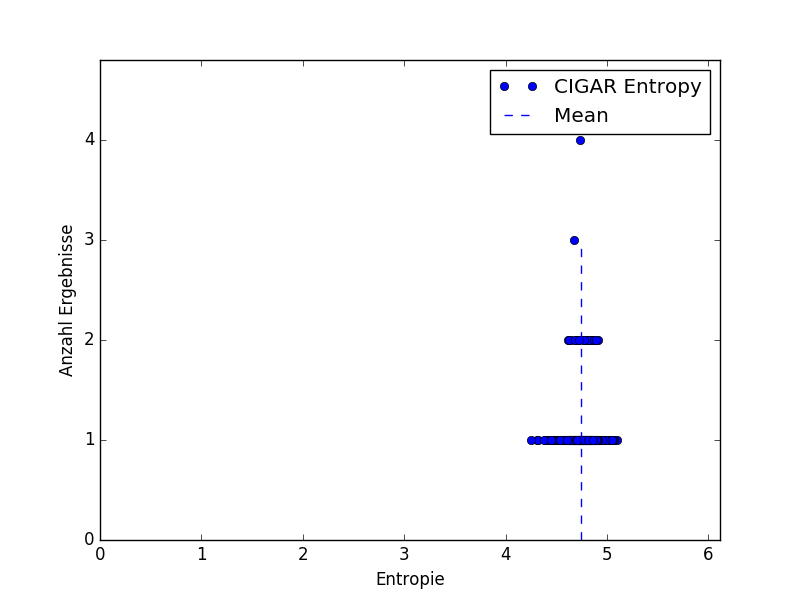
\includegraphics[width=12cm]{coding/cig_ent_einzel-1000-1000-d100}
	\caption{Entropie des CIGAR-Strings pro Symbol}
\end{figure}

\begin{figure}[h]
	\centering
	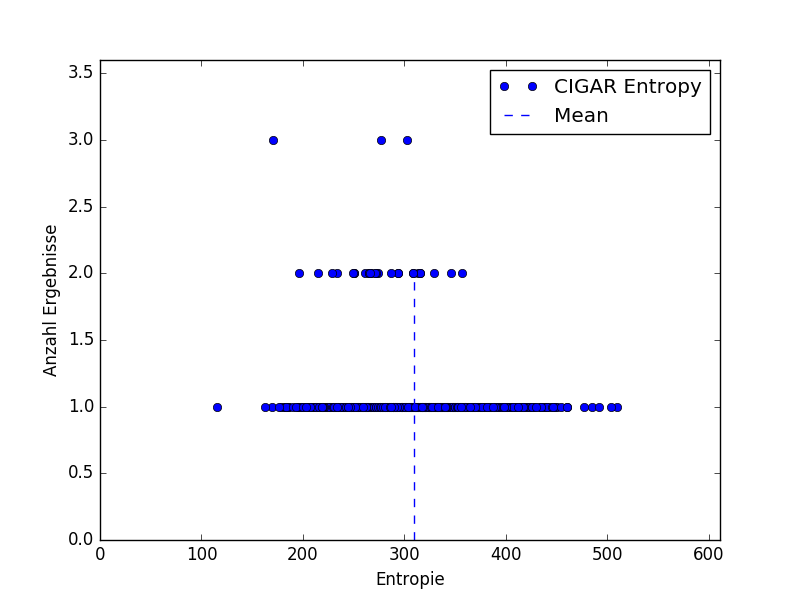
\includegraphics[width=12cm]{coding/cig_ent_faktor-1000-1000-d100}
	\caption{Entropie des CIGAR-Strings}
\end{figure}
\FloatBarrier
\subsection{Kodierung eines CIGAR-Strings}\label{Cigar_Beispiel}
Sei das Alignment $A$

\begin{verbatim}
0    5    0    5    0    5    0    5    0    
gagc-a-t-gttgcc-tggtcctttgctaggtactgta-gaga
|| | | | |  | | ||| |||| ||| ||| ||||| ||||
gaccaagtag--g-cgtggacctt-gctcggt-ctgtaagaga
0    5    0    5    0    5    0    5    0   
\end{verbatim}
gegeben, welches durch den CIGAR-String \texttt{4M1I1M1I1M1I1M2D1M1D1M1I8M\\1D7M1D5M1I4M} repr�sentiert werden kann.

Im Folgenden vergleiche ich f�r diese Art der Alignment-Repr�sentation die Verfahren der naiven bin�ren Kodierung, der un�ren Kodierung und der Huffman-Kodierung.

Sei das Alphabet $\cal{A}$$_1$ $= \{$M, I, D$\}$, welches alle Symbole aus dem CIGAR-String enth�lt, das Alphabet $\cal{A}$$_2$ $= \{1, 2, 4, 5, 7, 8\}$, welches alle Zahlen aus dem CIGAR-String enth�lt, sowie die relativen Wahrscheinlichkeiten $p(c_1)$ jeden Symbols $c_1 \in$ $\cal{A}$$_1$ und $p(c_2)$ jeden Symbols $c_2 \in$ $\cal{A}$$_2$ gegeben.

\begin{table}[h]
	\centering
	\begin{tabular}{cccc}
		$c_1$&H�ufigkeit&$p(c_1)$&\\
		\hline
		M & $10$ & $\frac{10}{38}$&\\
		I & $5$ & $\frac{5}{38}$&\\
		D & $4$ & $\frac{4}{38}$&\\
		&&&\\
		&&&\\
		&&&
	\end{tabular}\begin{tabular}{ccc}
	$c_2$&H�ufigkeit&$p(c_2)$\\
	\hline
	$1$ & $13$ &$\frac{13}{38}$\\
	$4$ & $2$ & $\frac{2}{38}$\\
	$2$ & $1$ & $\frac{1}{38}$\\
	$5$ & $1$ & $\frac{1}{38}$\\
	$7$ & $1$ & $\frac{1}{38}$\\
	$8$ & $1$ & $\frac{1}{38}$
\end{tabular}
\caption{Relative Wahrscheinlichkeiten CIGAR-String}
\end{table}

Bei einer naiven bin�ren Kodierung wird jedes Symbol $c_i \in \cal{A}$$_i$ mit $\lceil \log_2n
\rceil, n = |\cal{A}|$ Bit kodiert, also $\lceil \log_23\rceil + \lceil \log_26\rceil = 2 + 3 = 5$ Bit pro Symbol. Insgesamt ergibt das somit $19 \cdot 2 + 19 \cdot 3 = 95$ Bit.

Die un�re Kodierung kodiert jedes Symbol nach der H�ufigkeit des Auftretens im Alphabet mit $i - 1$ $'1'$-Bits, gefolgt von einem $'0'$-Bit, wobei $i$ die Position des Symbols in einer nach der H�ufigkeit absteigend sortierten Liste ist. Das am H�ufigsten auftretende Symbol des Alphabets wird also mit $'0'$, das zweith�ufigste mit $'10'$, das dritth�ufigste mit $'110'$ usw. kodiert. \cite[S. 29-30]{coding}

Der oben genannte CIGAR-String wird demnach wie folgt un�r kodiert:

\begin{table}[h]
	\centering
	\begin{tabular}{ccr}
		Symbol & Kodierung &  Anzahl Bits\\
		\hline
		M & $0$ & $10 \cdot 1 = 10$\\
		D & $10$ & $5 \cdot 2 = 10$\\
		I & $110$ & $4 \cdot 3 = 12$\\
		&&\\
		&&\\
		&&\\
		\hline
		\multicolumn{2}{l}{Gesamtanzahl:}&$32$
	\end{tabular}\begin{tabular}{ccr}
	Symbol & Kodierung &  Anzahl Bits\\
	\hline
	$1$ & $0$ & $13 \cdot 1 = 13$\\
	$4$ & $10$ & $2 \cdot 2 = \ \ 4$\\
	$2$ & $110$ & $1 \cdot 3 =\ \ 3$\\
	$5$ & $1110$ & $1 \cdot 4 =\ \ 4$\\
	$7$ & $11110$ & $1 \cdot 5 =\ \ 5$\\
	$8$ & $111110$ & $1 \cdot 6 =\ \ 6$\\
	\hline
	\multicolumn{2}{l}{}&$35$
\end{tabular}
\caption{Un�re Kodierung des CIGAR-Strings}
\end{table}

Insgesamt ben�tigt die un�re Kodierung also $32 + 35 = 67$ Bit.

Der durchschnittliche Bitverbrauch f�r ein Symbol betr�gt 
\[\frac{67}{38} \approx 1.76 \frac{\text{Bit}}{\text{Symbol}}\]

Bei einer \textit{minimalen} bin�ren Kodierung, wie sie auch im Huffman-Alogrithmus verwendet wird, werden die L�ngen der Codew�rter anhand der relativen Wahrscheinlichkeit des Symbols im Alphabet angepasst. Somit l�sst sich eine Kodierung erm�glichen, welche im Durchschnitt weniger Bit pro Symbol beansprucht \cite[S. 53-57]{coding}. Eine sparsamere Variante des regul�ren Huffman-Algorithmus ist der Kanonische Huffman-Algorithmus, welcher im Gegensatz zu der urspr�nglichen Variante eine eindeutige Menge von Codew�rtern liefert und keinen vollst�ndigen Huffman-Baum, sondern lediglich die Anzahl der Codew�rter f�r jede vorhandene Codewortl�nge, sowie die sortierten Symbole ben�tigt, um die Informationen zu dekodieren. %TODO cite und f�r Beispiele anwenden

Der Huffman-Algorithmus w�rde bei dem oben genannten Beispiel des CIGAR-Strings wie folgt ablaufen:

Ausf�hrung des Huffman-Algorithmus ergibt nach \cite[S. 54]{coding}:
\FloatBarrier
\begin{table}[h]
	\centering
	\begin{tabular}{ccr}
		Symbol & Kodierung & Anzahl Bits\\
		\hline
		M & $0$ & $10 \cdot 1 = 10$\\
		D & $10$ & $5 \cdot 2 = 10$\\
		I & $11$ & $4 \cdot 2 =\ \ 8$\\
		&&\\
		&&\\
		&&\\
		\hline
		\multicolumn{2}{l}{Gesamtanzahl:}&$28$
	\end{tabular}\begin{tabular}{ccr}
	Symbol & Kodierung & Anzahl Bits\\
	\hline
	$1$ & $00$ & $13 \cdot 2 = 26$\\
	$4$ & $01$ & $2 \cdot 2 =\ \ 4$\\
	$2$ & $100$ & $1 \cdot 3 =\ \ 3$\\
	$5$ & $101$ & $1 \cdot 3 =\ \ 3$\\
	$7$ & $110$ & $1 \cdot 3 =\ \ 3$\\
	$8$ & $111$ & $1 \cdot 3 =\ \ 3$\\
	\hline
	\multicolumn{2}{l}{}&$42$
\end{tabular}
\caption{Huffmann-Kodierung des CIGAR-Strings}
\end{table}
\FloatBarrier
und die dazugeh�rigen Huffman-B�ume:

\begin{figure}[h]
	\centering
	\begin{forest}
		for tree={grow'=south}
		[$\frac{19}{38}$
		[$\frac{9}{38}$, edge label={node[midway,right,font=\scriptsize]{1}}
		[I, edge label={node[midway,right,font=\scriptsize]{1}}]
		[D, edge label={node[midway,left,font=\scriptsize]{0}}] ] 
		[M, edge label={node[midway,left,font=\scriptsize]{0}}] ]
		]
	\end{forest}
	\begin{forest}
		for tree={grow'=south}
		[$\frac{19}{38}$
		[$\frac{4}{38}$, edge label={node[midway,right,font=\scriptsize]{1}}
		[$\frac{2}{38}$, edge label={node[midway,right,font=\scriptsize]{1}}
		[$8$, edge label={node[midway,right,font=\scriptsize]{1}}]
		[$7$, edge label={node[midway,left,font=\scriptsize]{0}}]]
		[$\frac{2}{38}$, edge label={node[midway,left,font=\scriptsize]{0}}
		[$5$, edge label={node[midway,right,font=\scriptsize]{1}}]
		[$2$, edge label={node[midway,left,font=\scriptsize]{0}}] ]]
		[$\frac{15}{38}$, edge label={node[midway,left,font=\scriptsize]{0}} 
		[$4$, edge label={node[midway,right,font=\scriptsize]{1}}]
		[$1$, edge label={node[midway,left,font=\scriptsize]{0}}] ]
		]
	\end{forest}
	\caption{Huffman-B�ume der Kodierung des CIGAR-Strings}
\end{figure}

Der gesamte Bitverbrauch dieser Kodierung ist demnach $28 + 42 = 70$ Bit.

Der durchschnittliche Bitverbrauch f�r ein Symbol betr�gt 
\[\frac{70}{38} \approx 1.84 \frac{\text{Bit}}{\text{Symbol}}\]

\section{TracePoint Konzept}

Ein neuer Ansatz der speichereffizienten Repr�sentation von Alignments wurde von Gene Myers in \cite{myers} beschrieben und basiert auf dem Konzept der Trace Points.

Sei $A$ ein Alignment von $u[i...j]$ und $v[k...\ell]$ mit $i < j$ und $k < l$ und sei $\Delta \in \mathbb{N}$. Sei $p = \left \lceil\frac{i}{\Delta}\right \rceil$. Man unterteilt $u[i...j]$ in $\tau = \left \lceil\frac{j}{\Delta}\right \rceil - \left \lfloor\frac{i}{\Delta}\right \rfloor$ Substrings $u_0, u_1, ... , u_{\tau -1}$ mit
\[  
u_q =
\begin{cases} 
u[i...p\cdot\Delta] & \text{falls }q = 0 \\
u[(p+q-1)\cdot\Delta+1...(p+q)\cdot\Delta] & \text{falls }0<q<\tau -1\\
u[(p+\tau-2)\cdot\Delta...j] & \text{falls }q = \tau -1
\end{cases}
\]

F�r alle $q$ mit $ 0 \leq q < \tau -1$ sei $t_q$ der letzte Index des Substrings von $v$, der in A mit $u_q$ aligniert. $t_q$ nennt man Trace Point. F�r $q = 0$ aligniert $u_0$ mit $v_0 = v[k...t_0]$. F�r alle $q$ mit $0<q< \tau -1$ aligniert $u_q$ mit $v_q = v[t_{q-1}+1...t_q]$.

Seien $i,j,k,\ell,\Delta$ und die Trace-Points eines Alignments von $u$ und $v$ gegeben. Dann kann ein Alignment $A'$ von $u$ und $v$ mit $\delta (A') \leq \delta (A)$ konstruiert werden. Danach bestimmt man aus den Trace-Points die Substring-Paare $u_q$ und $v_q$, berechnet hierf�r ein optimales Alignment und konkateniert die Alignments von den aufeinanderfolgenden Substring-Paaren zu $A'$.

Beispiel:
\begin{verbatim}
Sequenz 1: gagcatgttgcctggtcctttgctaggtactgtagaga
Sequenz 2: gaccaagtaggcgtggaccttgctcggtctgtaagaga
Delta: 15

Gesamtalignment:

0    5    0    5    0    5    0    5    0    
gagc-a-t-gttgcc-tggtcctttgctaggtactgta-gaga
|| | | | |  | | ||| |||| ||| ||| ||||| ||||
gaccaagtag--g-cgtggacctt-gctcggt-ctgtaagaga
0    5    0    5    0    5    0    5    0    



seq1[0...14] aligniert mit seq2[0...15]
gagc-a-t-gttgcc-tgg
|| | | | |  | | |||
gaccaagtag--g-cgtgg

seq1[15...29] aligniert mit seq2[16...28]
tcctttgctaggtac
|||| ||| ||| |
acctt-gctcggt-c

seq1[30...37] aligniert mit seq2[29...37]
tgta-gaga
|||| ||||
tgtaagaga

Trace Points: [15, 28] 
\end{verbatim}

\subsection{Komplexit�t}

TODO

%TODO ausf�hrlicher
F�r die Trace-Point Repr�sentation wird f�r eine Edit-Distanz $e$ mit Einheitskosten als Kostenfunktion $\delta$ wie oben beschrieben lediglich $O(e^2)$ Zeit pro Teilalignment ben�tigt, wobei bei einer erwarteten Fehlerrate $\varepsilon$ des Alignments die Edit-Distanz immer h�chstens so gro� ist wie die Anzahl der Fehler im Teilalignment. \cite[S.41-42]{gsa-skript}

\subsection{Speicherverbrauch}

%TODO
\subsection{Entropie unabh�ngig vom Kodierungsverfahren}

\begin{figure}[h]
	\centering
	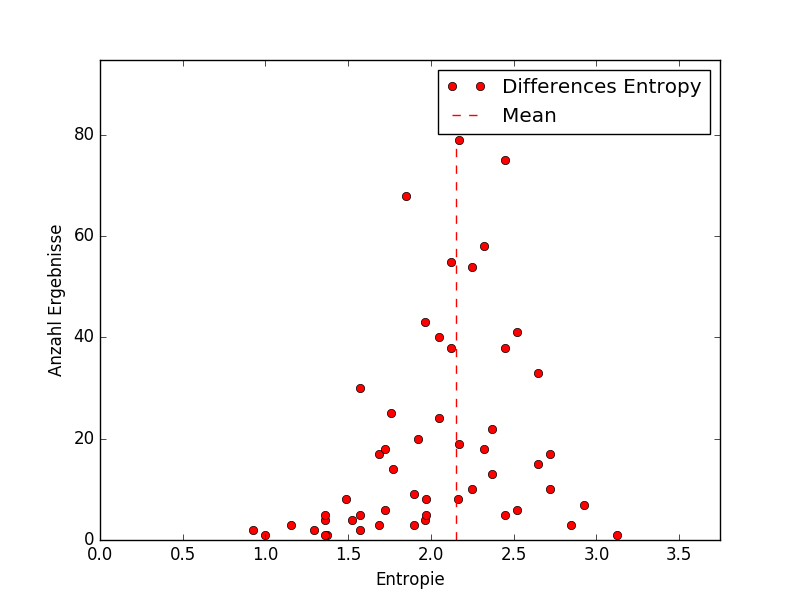
\includegraphics[width=12cm]{coding/diff_ent_einzel-1000-1000-d100}
	\caption{Entropie des CIGAR-Strings pro Symbol}
\end{figure}

\begin{figure}[h]
	\centering
	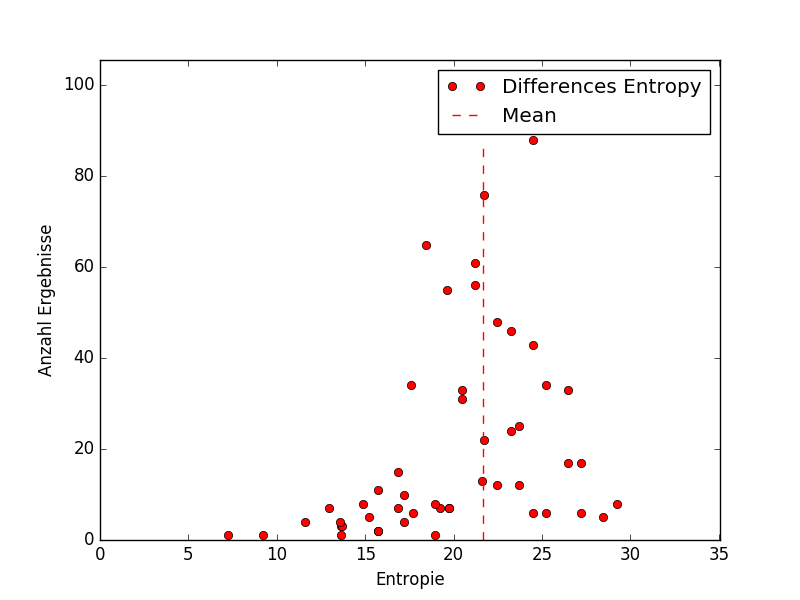
\includegraphics[width=12cm]{coding/diff_ent_faktor-1000-1000-d100}
	\caption{Entropie des CIGAR-Strings}
\end{figure}
\FloatBarrier
\section{Differenzen-Kodierung}\label{Differenzen-Kodierung}

%TODO Quellen
Gegeben sei eine Liste $L = (a_1, a_2, ... , a_n)$ mit $a_i < a_{i+1}, 0 < i \leq n$.

Anstatt jeden Wert $a \in L$ als solchen abzuspeichern, kann alternativ die Differenz eines Wertes $a_i$ zu dem nachfolgenden Wert $a_{i+1}$ abgespeichert werden. Lediglich der erste (oder letzte) Wert aus $L$ wird ben�tigt, um sp�ter sukzessive die urspr�ngliche Liste rekonstruieren zu k�nnen.
\[L_{diff} = (a_1, (a_2-a_1), (a_3-a_2), ... , (a_{n}-a_{n-1}))\]

Bei gleichm��ig ansteigenden Werten ist die Abweichung der Differenzen zweier aufeinanderfolgender Werte in der Liste untereinander gering und die Menge der zu kodierenden Symbole verringert sich.

\subsection{Kodierung der Trace Point Differenzen}
Sei $\Delta = 5$ und das Alignment $A$
\begin{verbatim}
0    5    0    5    0    5    0    5    0    
gagc-a-t-gttgcc-tggtcctttgctaggtactgta-gaga
|| | | | |  | | ||| |||| ||| ||| ||||| ||||
gaccaagtag--g-cgtggacctt-gctcggt-ctgtaagaga
0    5    0    5    0    5    0    5    0   
\end{verbatim}

wie in Abschnitt \ref{Cigar_Speicher} mit den dazugeh�rigen TracePoints $5, 10, 15, 20, 24, 28$ und $34$ gegeben. Es ergibt sich somit das Alphabet $\cal{A}$ $= \{5, 10, 15, 20, 24, 28, 34\}$ mit ausschlie�lich positiven und aufsteigenden Werten.

F�r die Trace Point Darstellung ist somit eine Differenzen-Kodierung m�glich. Als neue Liste zu kodierender Werte ergibt sich nach \ref{Differenzen-Kodierung} $L_{diff} = (5, 5, 5, 5, 4, 4, 6)$.

Um aus den Trace Points ein neues Alignment rekonstruieren zu k�nnen, ben�tigt man zus�tzlich mindestens den $\Delta$-Wert, damit die Grenzen der Substrings beider Sequenzen berechnet werden k�nnen. Hierf�r muss also der $\Delta$-Wert zu $L$ hinzugef�gt werden.

F�r das oben genannten Beispiel ergibt sich somit $L_{diff} = (5, 5, 5, 5, 5, 4, 4, 6)$.

Sei das Alphabet $\cal{A}$ $= \{4, 5, 6\}$ f�r $L_{diff}$, sowie die relativen Wahrscheinlichkeiten $p(c)$ jeden Symbols $c \in$ $\cal{A}$ gegeben. 

\begin{table}[h]
	\centering
	\begin{tabular}{ccc}
		$c$&H�ufigkeit&$p(c)$\\
		\hline
		$5$ & $5$ & $\frac{5}{8}$\\
		$4$ & $2$ & $\frac{2}{8}$\\
		$6$ & $1$ & $\frac{1}{8}$
	\end{tabular}
	\caption{Relative Wahrscheinlichkeiten der Delta-Kodierung}
\end{table}

Bei der naiven bin�ren Kodierung ergibt sich analog zu \ref{Cigar_Speicher} ein Bedarf von $\lceil \log_28\rceil = 3$ Bit pro Symbol, also $8 \cdot 3 = 24$ Bit insgesamt.

Die un�re Kodierung ergibt f�r dieses Beispiel die folgende Kodierung:

\begin{table}[h]
	\centering
	\begin{tabular}{ccr}
		Symbol & Kodierung &  Anzahl Bits\\
		\hline
		$5$ & $0$ & $5 \cdot 1 = 5$\\
		$4$ & $10$ & $2 \cdot 2 = 4$\\
		$6$ & $110$ & $1 \cdot 3 = 3$\\
		\hline
		\multicolumn{2}{l}{Gesamtanzahl:}&$12$
	\end{tabular}
	\caption{Un�re Kodierung der Delta-Kodierung}
\end{table}

Insgesamt ben�tigt die un�re Kodierung also $12$ Bit mit einem durchschnittlichen Verbrauch pro  Symbol von
\[\frac{12}{8} \approx 1.5 \frac{\text{Bit}}{\text{Symbol}}\]

Die Ausf�hrung des Huffman-Algorithmus ergibt nach \cite[S. 54]{coding}:

\begin{table}[h]
	\centering
	\begin{tabular}{ccr}
		Symbol & Kodierung & Anzahl Bits\\
		\hline
		$5$ & $0$ & $5 \cdot 1 = 5$\\
		$4$ & $10$ & $2 \cdot 2 = 4$\\
		$6$ & $11$ & $1 \cdot 2 = 2$\\
		\hline
		\multicolumn{2}{l}{Gesamtanzahl:}&$11$
	\end{tabular}
	\caption{Huffman-Kodierung der Delta-Kodierung}
\end{table}

\FloatBarrier

und der dazugeh�rige Huffman-Baum:

\begin{figure}[h]
	\centering
	\begin{forest}
		for tree={grow'=south}
		[$\frac{8}{8}$
		[$\frac{3}{8}$, edge label={node[midway,right,font=\scriptsize]{1}}
		[$6$, edge label={node[midway,right,font=\scriptsize]{1}}]
		[$4$, edge label={node[midway,left,font=\scriptsize]{0}}]]
		[$5$, edge label={node[midway,left,font=\scriptsize]{0}}]
		]
	\end{forest}
	\caption{Huffman-Baum der Delta-Kodierung}
\end{figure}

Der gesamte Bitverbrauch der Huffman-Kodierung ist demnach $11$ Bit mit einem durchschnittlichen Verbrauch pro Symbol von 
\[\frac{11}{8} \approx 1.38 \frac{\text{Bit}}{\text{Symbol}}\]

\chapter{Resultate}
%TODO hier soll neutral und ohne Wertung beschrieben werden, was in den Testl�ufen herausgekommen ist. Die ganzen Grafiken sollen hier gezeigt werden

\section{Testl�ufe CIGAR Kodierung}\label{Cigar_Testl�ufe}

Die folgenden Grafiken wurden mit jeweils 10.000 zuf�llig generierte Sequenzpaaren mit je etwa 1.000 Basen, einer Fehlerrate von 15\% und einem $\Delta$-Wert von 100 berechnet.

\begin{figure}[h]
	\centering
	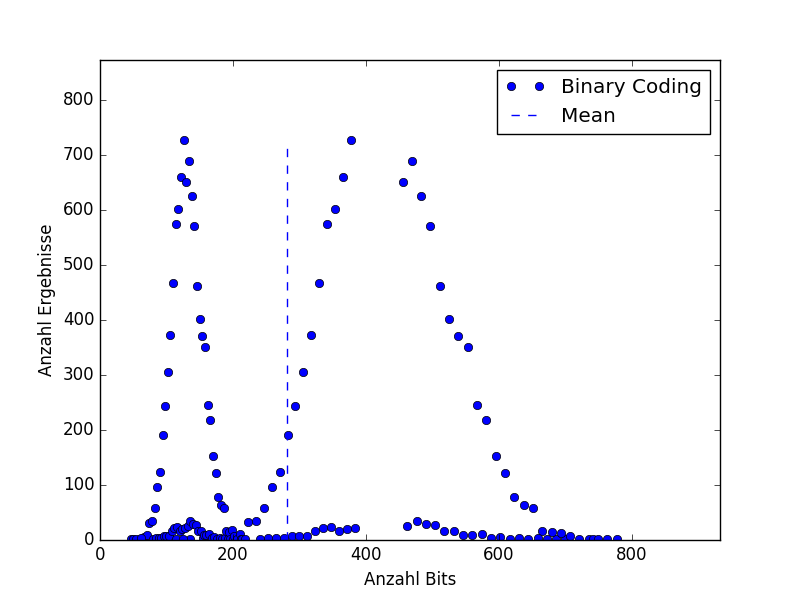
\includegraphics[width=12cm]{coding/cig-bin-10000-1000-d100}
	\caption{Bitverbrauch der bin�ren Kodierung des CIGAR-Strings}\label{fig:cig-bin}
\end{figure}

\begin{figure}[h]
	\centering
	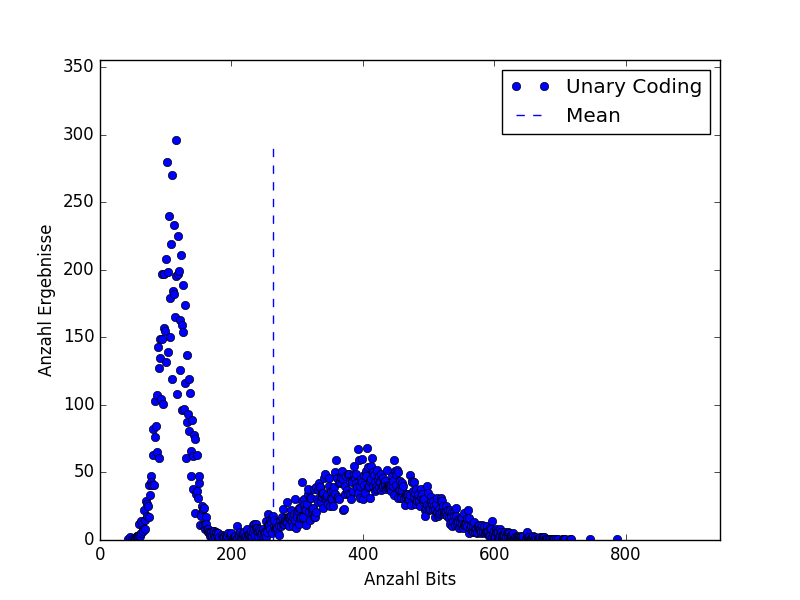
\includegraphics[width=12cm]{coding/cig-una-10000-1000-d100}
	\caption{Bitverbrauch der un�ren Kodierung des CIGAR-Strings}\label{fig:cig-una}
\end{figure}

\begin{figure}[h]
	\centering
	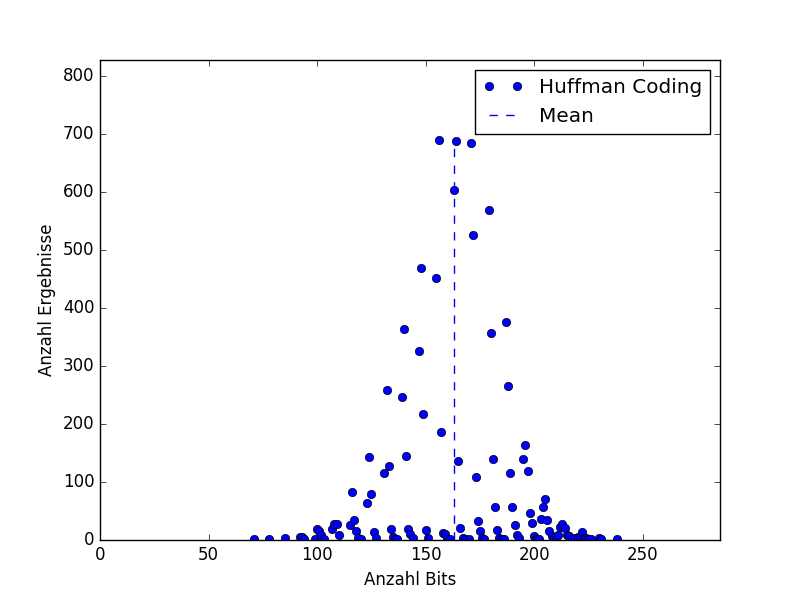
\includegraphics[width=12cm]{coding/cig-huf-10000-1000-d100}
	\caption{Bitverbrauch der Huffman-Kodierung des CIGAR-Strings}\label{fig:cig-huf}
\end{figure}

Die Abbildungen \ref{fig:cig-bin} und \ref{fig:cig-una} verdeutlichen, dass die bin�re und un�re Kodierung deutliche Schwankungen im Bitverbrauch aufweisen, welche sich durch die zuf�llig generierten Sequenzpaare erkl�ren lassen, deren Alignments unter Umst�nden sehr viele oder ausschlie�lich Matches bzw. sehr viele InDels aufweisen k�nnen. Die Abbildung \ref{fig:cig-huf} hingegen weist eine Normalverteilung des Bitverbrauchs f�r die Huffman-Kodierung auf.
Im Mittel ben�tigt die naive bin�re Kodierung $284.60$ Bit, die un�re Kodierung $264.84$ Bit und die Huffman-Kodierung $162.93$ Bit.

In den dargestellten Testl�ufen verbraucht die Huffman-Kodierung somit durchschnittlich mit Abstand am wenigsten Speicher, obwohl in dem unter \ref{Cigar_Beispiel} beschriebenen Beispiel die un�re Kodierung den CIGAR-String etwas effizienter kodiert. Der Grund hierf�r ist die deutlich h�here Fehlerrate in \ref{Cigar_Beispiel}, welche die Anzahl der zu kodierenden Symbole deutlich erh�ht.

Das CIGAR-Format ben�tigt folglich wenig Speicher f�r Alignments mit einer kleinen Edit-Distanz und deutlich mehr Speicher f�r Alignments mit einer gro�en Edit-Distanz, da in diesem Fall eine h�here Anzahl unterschiedlicher Symbole kodiert werden muss.

\section{Testl�ufe Differenzen Kodierung}\label{Diff-Testl�ufe}

Die folgenden Grafiken wurden mit jeweils 10.000 zuf�llig generierte Sequenzpaaren mit je etwa 1.000 Basen, einer Fehlerrate von 15\% und einem $\Delta$-Wert von 100 berechnet.

\begin{figure}[h]
	\centering
	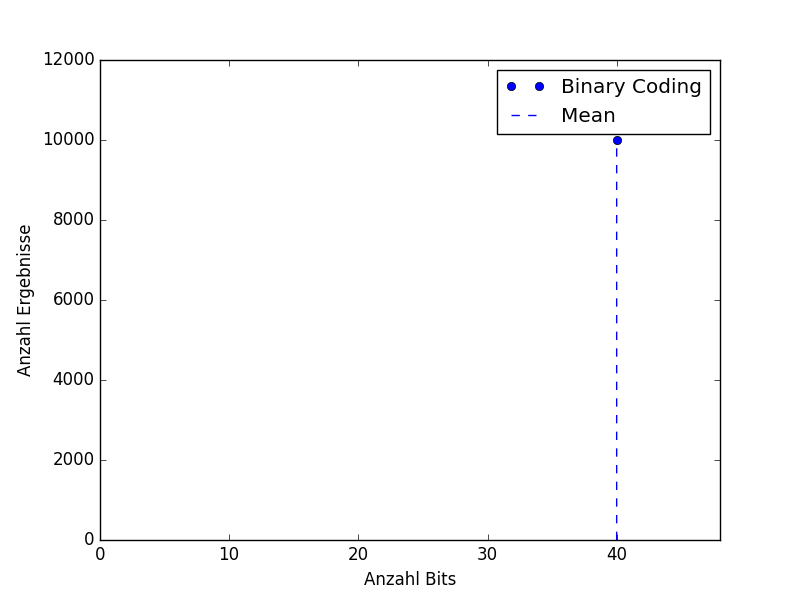
\includegraphics[width=12cm]{coding/diff-bin-10000-1000-d100}
	\caption{Bitverbrauch der naiven bin�ren Kodierung der Delta-Kodierung}\label{fig:diff-bin}
\end{figure}

\begin{figure}[h]
	\centering
	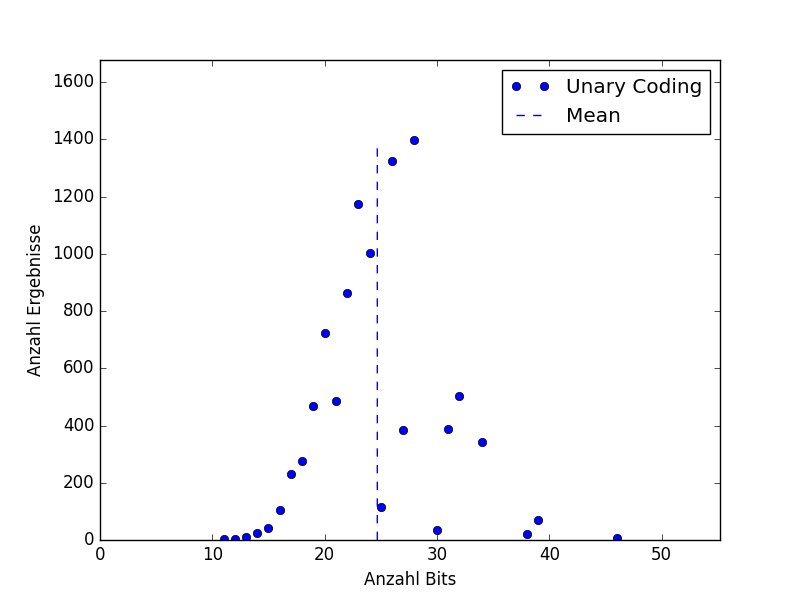
\includegraphics[width=12cm]{coding/diff-una-10000-1000-d100}
	\caption{Bitverbrauch der un�ren Kodierung der Delta-Kodierung}\label{fig:diff-una}
\end{figure}

\begin{figure}[h]
	\centering
	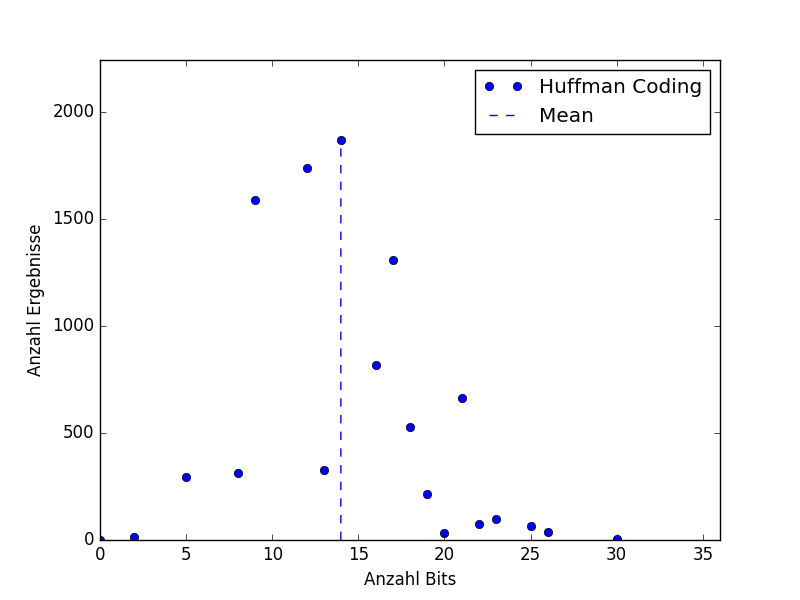
\includegraphics[width=12cm]{coding/diff-huf-10000-1000-d100}
	\caption{Bitverbrauch der Huffman-Kodierung der Delta-Kodierung}\label{fig:diff-huf}
\end{figure}

Die naive bin�re Kodierung ben�tigt, wie in Abbildung \ref{fig:diff-bin} dargestellt, in jedem Durchlauf und somit auch im Mittel konstant $40$ Bit, da f�r jeden Durchlauf $9$ Trace Points und der $\Delta$-Wert gespeichert werden f�r $\lceil \log_210 \rceil \cdot 10 = 40$ Bit.

Die Abbildungen \ref{fig:diff-una} verdeutlicht, dass die un�re Kodierung Schwankungen im Bitverbrauch aufweist, welche sich wie bei den CIGAR-Strings durch die zuf�llig generierten Sequenzpaare erkl�ren lassen, deren Alignments unter Umst�nden sehr viele oder ausschlie�lich Matches bzw. sehr viele InDels aufweisen k�nnen. Sie ben�tigt im Mittel $24.70$ Bit und damit nur etwa $62$\% der bin�ren Kodierung.

F�r die Huffman-Kodierung wird, wie in Abbildung \ref{fig:diff-huf} zu sehen ist, deutlich weniger Speicher f�r die Kodierung ben�tigt als f�r die naive bin�re oder un�re Kodierung. Sie verbraucht durchschnittlich nur $14.00$ Bit und damit nur etwa $57$\% des Speicherbedarfs der un�ren Kodierung.

Es ist somit zu erkennen, dass die Kodierung der Differenzen der Trace Points mit den oben genannten Parametern der Testl�ufe in allen Kodierungen weniger Speicher ben�tigt, als die Kodierung eines CIGAR-Strings, wobei die Huffman-Kodierung mit Abstand am effizientesten ist. Hierbei ist jedoch zu beachten, dass der Speicherverbrauch der Trace Point Kodierung von der Wahl des $\Delta$-Wertes abh�ngt, da bei einem kleinen $\Delta$ mehr Trace Points und somit mehr Symbole gespeichert werden m�ssen, als bei einem gro�en $\Delta$-Wert.

\chapter{Diskussion}
%TODO hier soll wertend beschrieben werden, was die Resultate bedeuten und wie sich bestimmte Werte erkl�ren lassen
\section{Bewertung CIGAR-Kodierung}
\section{Bewertung Differenzen-Kodierung der Trace Points}

\chapter{Programm}

\section{Aufbau}
\begin{figure}[h]
	\centering
	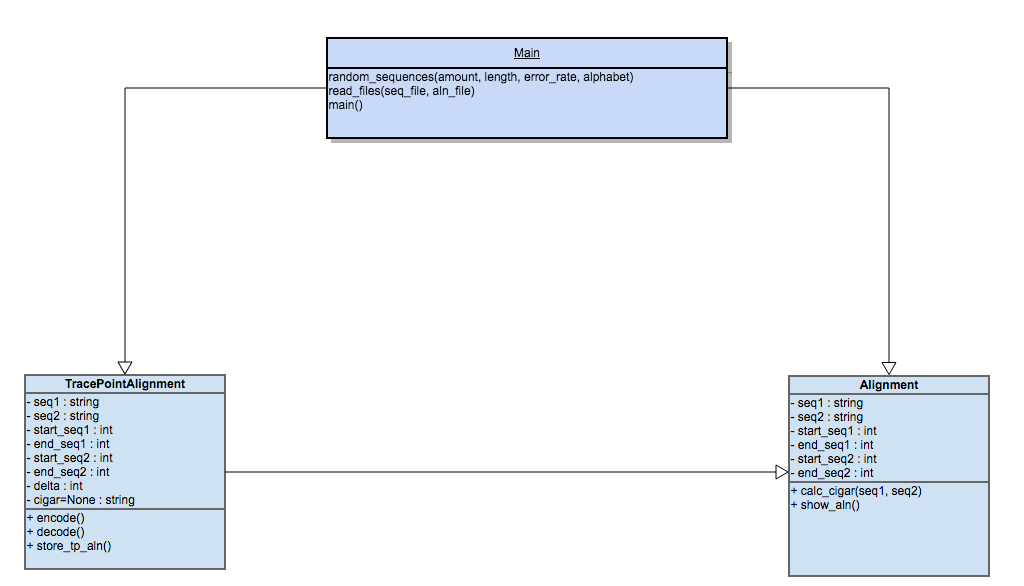
\includegraphics[width=\textwidth]{images/UML}
	\caption{UML-Diagramm}
\end{figure}

\clearpage

\section{Funktionalit�t}

\begin{algorithm}[h]
	\caption{Computation of Trace Points from a given CIGAR-String}
	\label{encode}
	\noindent\begin{tabular}{@{}l@{~}l}
		\textbf{Input}:
		&$seq1, seq2, start\_seq1, end\_seq1, start\_seq2, \Delta, cigar$ mit \\
		&$\Size{seq1}, \Size{seq2}, \Size{cigar} > 0$;\\
		&$start\_seq1, start\_seq2 \geq 0$;\\
		&$start\_seq1 < end\_seq1$ und\\
		&$\Delta > 0$\\
		\textbf{Output}:&Array $TP$ of Trace Points
	\end{tabular}
	\medskip
	\begin{algorithmic}[1]
		\Function{\textit{encode}}{$seq1, seq2, start\_seq1, end\_seq1, start\_seq2, \Delta, cigar$}
		\State \Assign{itv\_size}{MAX(1, \Roundup{start\_seq1/\Delta})}
		\State \Assign{itv\_count}{MIN(\Roundup{\Size{seq1}/\Delta}, \Roundup{\Size{seq2}/\Delta})}
		\For{\Assign{i}{0} \Upto \(\Size{itv\_count}\)} \\
		\Assign{\indent itv[i]}{
			\begin{cases}
				start\_seq1, itv\_size \cdot \Delta - 1&\text{ if } i = 0\\
				(itv\_size + i - 1) \cdot \Delta, (itv\_size + i) \cdot \Delta - 1&\text{ if } 0 < i < \Size{itv\_count}\\
				(itv\_size + i - 1) \cdot \Delta, end\_seq1 - 1&\text{ else.}
			\end{cases}}
			\EndFor
			\State \Assign{count1, count2, count3}{0}
			\State \Assign{TP}{\text{Array for Trace Points}}
			\For{\text{each $(cig\_count, cig\_symbol)$ in cigar}}
			\For{\Assign{i}{0} \Upto \(cig\_count\)}
			\If{cig\_symbol = 'I'}
			\State increment $count1$
			\ElsIf{cig\_symbol = 'D'}
			\State increment $count2$
			\Else
			\State increment $count1, count2$
			\EndIf
			
			\If{count1 = intervals[count3][1] + 1 \textbf{and} count1 $\neq \Size{seq1}$}
			\State append (count2 - 1 + start\_seq2) to $TP$
			\EndIf
			\If{count $\neq \Size{itv} - 1$}
			\State increment $count3$
			\EndIf
			\EndFor
			\EndFor
			\State \Return $TP$
			\EndFunction
		\end{algorithmic}
	\end{algorithm}
	
	\FloatBarrier
	\subsection{Informationsverlust bei der encode()-Funktion}
	Die encode-Funktion extrahiert aus dem gegebenen CIGAR-String die Trace Points, welche dann zusammen mit dem $\Delta$-Wert und den Start- und Endpositionen der Sequenzabschnitte gespeichert werden. Hierbei geht die Information, wie die jeweiligen Intervalle zwischen den Trace Points zu den komplement�ren Intervallen in der Ursprungssequenz aligniert werden, verloren.
	F�r die R�ckgewinnung dieser Information muss in der decode()-Funktion zun�chst ein neues Alignment des jeweiligen Intervall-Paares errechnet werden und alle Teilalignments zu einem Gesamtalignment konkateniert werden.
	
	\begin{algorithm}[h]
		\caption{Computation of a CIGAR-String from a given Trace Point Array}
		\label{decode}
		\noindent\begin{tabular}{@{}l@{~}l}
			\textbf{Input}:
			&$seq1, seq2, \Delta, TP$ mit\\
			&$\Size{seq1}, \Size{seq2}, \Delta, \Size{TP} > 0$\\
			\textbf{Output}:&CIGAR-String
		\end{tabular}
		\medskip
		\begin{algorithmic}[1]
			\Function{\textit{decode}}{$seq1, seq2, \Delta, TP$}
			\State \Assign{cig}{\text{empty String}}
			\For{\Assign{i}{0} \Upto \(\Size{TP}\)}
			\If{i = 0}
			\State append \textbf{cigar}($seq1[0...\Delta], seq2[0...TP[i] + 1]$) to $cig$
			\ElsIf{i = \Size{TP} - 1}
			\State append \textbf{cigar}($seq1[i \cdot \Delta...\Size{seq1}], seq2[TP[i - 1] + 1...\Size{seq2}]$) to $cig$
			\Else
			\State \begin{tabular}{rll}
				append \textbf{cigar}&($seq1[i \cdot \Delta...(i + 1) \cdot \Delta],$&\\
				&$seq2[TP[i - 1] + 1]...TP[i] + 1$)& to $cig$
			\end{tabular}
			
			\EndIf
			\EndFor
			\State \Assign{cig}{\textbf{combine}(cig)}
			\State \Return cig
			\EndFunction\\
			
			\Function{\textit{combine}}{$cigar$}
			\State \Assign{cig}{\text{empty String}}
			\State \Assign{tmp}{0}
			\For{\text{each $(cig\_count, cig\_symbol)$ in cigar}}
			\State \Assign{tmp}{tmp + previous\_cig\_count}
			\If{cig\_symbol = previous\_cig\_symbol}
			\If{\text{not last element in cigar}}
			\State \Assign{tmp}{0}
			\EndIf
			\EndIf
			\If{\text{last element in cigar}}
			\State \text{append $(tmp + cig\_count, cig\_symbol)$ to cig}
			\EndIf
			\EndFor
			\State \Return cig
			\EndFunction
		\end{algorithmic}
	\end{algorithm}
	
\chapter{Fazit}

Je gr��er der vorher definierte positive Parameter $\Delta$ ist, desto weniger Trace Points werden gespeichert und umso l�nger dauert die Berechnung, um die Teil-Alignments zu rekonstruieren. Bei einem kleinen $\Delta$ werden analog mehr Trace Points gespeichert, aber die Rekonstruktionszeit der Teil-Alignments ist geringer.

Mithilfe von $\Delta$ l�sst sich somit ein Trade-Off zwischen dem Speicherplatzverbrauch und dem Zeitbedarf f�r die Rekonstruktion der Teil-Alignments einstellen.
\cleardoublepage

% Anhang
%\appendix
%%
% Anhang
%

\chapter{Anhang}
Lorem ipsum dolor sit amet, consectetuer adipiscing elit. Cras semper. Integer sapien nulla, consectetuer a, laoreet et, varius quis, mauris. Nunc pharetra tincidunt massa. Pellentesque habitant morbi tristique senectus et netus et malesuada fames ac turpis egestas. Praesent pellentesque mauris at elit. Aliquam consequat suscipit enim. Pellentesque habitant morbi tristique senectus et netus et malesuada fames ac turpis egestas. Nunc sapien. Proin hendrerit diam at quam. Lorem ipsum dolor sit amet, consectetuer adipiscing elit. Integer vulputate semper nunc. Sed dui. Praesent at sem. Integer elit ipsum, placerat vitae, dictum quis, feugiat sit amet, metus.

\section{�berschrift zweiter Ordnung}
Donec arcu turpis, pretium quis, interdum non, condimentum a, est. Fusce lobortis urna non tellus. Nam leo dui, malesuada non, tempus placerat, congue eget, pede. Mauris porttitor risus quis tortor molestie vehicula. Curabitur tincidunt. In malesuada congue nisi. Nullam et nulla. Curabitur porttitor. Ut molestie sagittis felis. Sed urna libero, ultricies quis, laoreet eget, congue id, metus. Proin ac lorem cursus mauris auctor laoreet. Donec justo. Etiam nunc sem, dapibus sit amet, euismod a, molestie sit amet, mi.

Morbi sollicitudin consequat magna. Vivamus dictum. Nulla non quam. Nam sem tellus, aliquam sed, hendrerit nec, imperdiet ut, augue. Aliquam erat volutpat. Vivamus non ligula sit amet lorem accumsan viverra. Cras mattis libero et ante. Cras massa. Donec fringilla, metus vitae semper condimentum, dolor dui fringilla arcu, et mattis nulla dui vel lectus. Nunc mauris magna, tristique eu, rutrum at, facilisis eu, odio. Nullam congue magna non nisi. Suspendisse viverra, massa non pellentesque scelerisque, risus elit 

\noindent Hier kommt ein Listing \ref{lst:soap}.

\begin{center}
\begin{lstlisting}[caption={SOAP Anfrage an einen HalloWelt-Web-Service},label=lst:soap,language=XML,label={lst:soap}]
<?xml version='1.0' encoding='UTF-8'>
<SOAP-ENV:Envelope (*@\label{lst:soapEnv}@*)
  xmlns:SOAP-ENV="http://schemas.xmlsoap.org/soap/envelope/"
  xmlns:xsi="http://www.w3.org/2001/XMLSchema-instance"
  xmlns:xsd="http://www.w3.org/2001/XMLSchema"
  xmlns:ns1="http://localhost/wsdl/HalloWeltService.wsdl">
  
  <SOAP-ENV:Body>(*@\label{lst:soapBody}@*)
  	<ns1:gruss>
  		<name xsi:type="xsd:string">
  			Michael
  		</name>
  	</ns1:gruss>
  </SOAP-ENV:Body>

</SOAP-ENV:Envelope>
\end{lstlisting}
\end{center}

bibendum dolor, vitae ultrices lorem neque et erat. Nullam tortor ante, venenatis et, aliquet ac, ornare id, massa. Vivamus urna augue, posuere vitae, sagittis id, porttitor at, arcu. Praesent pharetra rutrum neque. Maecenas tempor ultrices felis.
Nulla facilisi. In sed elit aliquet neque malesuada blandit. Nam tempus imperdiet eros. Mauris tincidunt diam eu erat. Phasellus iaculis blandit leo. Nunc augue. Donec dignissim accumsan pede. Ut consequat, eros id accumsan placerat, mi justo ullamcorper pede, id lacinia augue nisi non nibh. Vestibulum eget arcu. Cras pretium, dui eu gravida varius, lectus neque accumsan ligula, eu sodales magna lectus ut nisi. Aliquam vel ante. Ut suscipit porta augue. Suspendisse pellentesque faucibus nisl. Nulla magna tortor, cursus quis, varius quis, hendrerit ut, neque.


%
% EOF
%
%\cleardoublepage

\phantomsection % ben�tigt f�r korrekte pdf-darstellung
\addcontentsline{toc}{chapter}{Literaturverzeichnis}
\bibliographystyle{natdin} % Din 1505 nach Lorenzen (Das konkrete Aussehen des Litverzeichnisses ist im header festgelegt)
\bibliography{bibliography/literatur}  % Pfad zur *.bib-Datei (Dateiendung wird weggelassen)
\cleardoublepage

\chapter*{Eidesstattliche Erkl�rung}
\thispagestyle{empty}
\addcontentsline{toc}{chapter}{Eidesstattliche Erkl�rung}

Ich versichere, dass ich die vorstehende Arbeit selbstst�ndig und ohne fremde Hilfe angefertigt und mich anderer als der im beigef�gten Verzeichnis angegebenen Hilfsmittel nicht bedient habe. Alle Stellen, die w�rtlich oder sinngem�� aus Ver�ffentlichungen entnommen wurden, sind als solche kenntlich gemacht. \\

%\noindent Ich bin mit einer Einstellung in den Bestand der Bibliothek des Fachbereiches einverstanden.

\vspace{2cm} 

\noindent Hamburg, den \uline{~~~~~~~~~~~~~~~~~~~~}~~~~~Unterschrift: \uline{~~~~~~~~~~~~~~~~~~~~~~~~~~~~~~~~~~~~~~~~~~~~~~~~~~} 


\end{document}
